\documentclass[a4paper,11pt]{jsarticle}

% --- パッケージのロード ---
\usepackage[dvipdfmx]{graphicx}
\usepackage[utf8]{inputenc}
\usepackage{amsmath, amssymb}
\usepackage{geometry}
\usepackage{listings}
\usepackage{xcolor}
\usepackage{bm}
\usepackage{float}

% ページ設定
\geometry{left=20mm,right=20mm,top=25mm,bottom=25mm}

% ソースコード表示用設定
\lstset{
    basicstyle=\ttfamily\small,
    frame=single,
    breaklines=true,
    backgroundcolor=\color{gray!5},
    keywordstyle=\color{blue},
    commentstyle=\color{green!50!black},
    stringstyle=\color{red},
    numbers=left,
    numberstyle=\tiny\color{gray},
    stepnumber=1,
    captionpos=b
}

\title{課題09-1 レポート}
\date{\today}

\begin{document}

\maketitle

\section{System 2}

\subsection{a. システムの伝達関数の決定}
提供されたSystem 2のステップ応答グラフを観察すると、入力 $u(t) = 1$（単位ステップ入力）に対して、出力 $y(t)$ が時間 $t$ に比例して直線的に増加していることがわかる。
グラフより、$t = 10$ のとき $y(10) = 100$ である。このことから、出力は以下の式で表される：
\begin{equation}
    y(t) = 10t
\end{equation}
これをラプラス変換すると、$Y(s) = \frac{10}{s^2}$ となる。入力 $U(s) = \frac{1}{s}$ であるから、伝達関数 $G(s)$ は次のように求められる：
\begin{equation}
    G(s) = \frac{Y(s)}{U(s)} = \frac{10/s^2}{1/s} = \frac{10}{s}
\end{equation}
したがって、System 2は積分要素であり、ゲインは10である。

\subsection{b. 伝達関数の導出方法の説明}
導出の手順は以下の通りである：
\begin{enumerate}
    \item \textbf{定常状態の確認：} ステップ応答が一定値に収束せず、一定の傾きで増加し続けていることから、システムに積分器（$1/s$）が含まれていると判断した。
    \item \textbf{傾きの算出：} グラフ上の2点 $(0, 0)$ および $(10, 100)$ を結ぶ直線の傾き $K$ を算出した。$K = \frac{100 - 0}{10 - 0} = 10$。
    \item \textbf{時間領域から複素領域への変換：} 単位ステップ応答 $y(t) = Kt$ の関係から、伝達関数 $G(s) = \frac{K}{s}$ を導いた。
\end{enumerate}

\newpage

\section{System 7 の解析（2次系・2重積分要素）}

\subsection{a. システムの伝達関数の決定}
System 7のステップ応答グラフを観察すると、出力 $y(t)$ は放物線状（時間の2乗に比例）に増加している。
グラフより、$t = 10$ のとき $y(10) = 300$ である。
一般に、2重積分要素のステップ応答は $y(t) = \frac{K}{2}t^2$ と表される。
$300 = \frac{K}{2}(10)^2$ より、$300 = 50K$、すなわち $K = 6$ である。
したがって、$y(t) = 3t^2$ であり、これをラプラス変換すると $Y(s) = \frac{3 \cdot 2!}{s^3} = \frac{6}{s^3}$ となる。
入力 $U(s) = 1/s$ より、伝達関数 $G_7(s)$ は以下の通りとなる。
\begin{equation}
    G_7(s) = \frac{6/s^3}{1/s} = \frac{6}{s^2}
\end{equation}

\subsection{b. 伝達関数の導出方法の説明}
\begin{enumerate}
    \item \textbf{特性の判別：} 出力曲線が $t=0$ で傾き0から始まり、加速するように増加していることから、2重積分特性 ($1/s^2$) を持つ2次系と判断した。
    \item \textbf{ゲインの算出：} $y(t) = \frac{K}{2}t^2$ のモデルを適用し、$t=10, y=300$ を代入してゲイン $K=6$ を得た。
\end{enumerate}

\subsection{c. シミュレーションによる検証}

\begin{figure}[H]
    \centering
    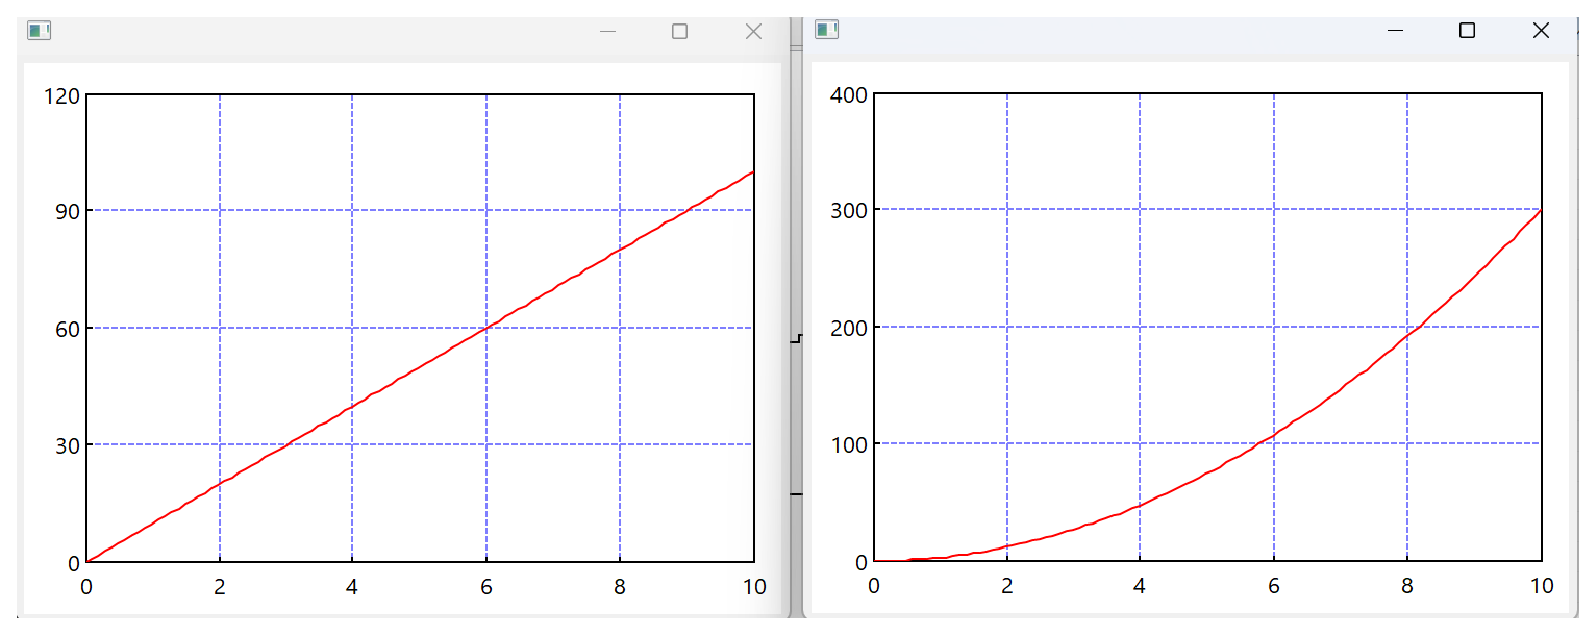
\includegraphics[width=0.8\columnwidth]{picture1.eps}
    \caption{picture1の画像}
    \label{fig:picture1}
\end{figure}

\end{document}